\documentclass[journal,12pt,twocolumn]{IEEEtran}

\usepackage{setspace}
\usepackage{gensymb}

\singlespacing


\usepackage[cmex10]{amsmath}

\usepackage{amsthm}

\usepackage{mathrsfs}
\usepackage{txfonts}
\usepackage{stfloats}
\usepackage{bm}
\usepackage{cite}
\usepackage{cases}
\usepackage{subfig}

\usepackage{longtable}
\usepackage{multirow}

\usepackage{enumitem}
\usepackage{mathtools}
\usepackage{steinmetz}
\usepackage{tikz}
\usepackage{circuitikz}
\usepackage{verbatim}
\usepackage{tfrupee}
\usepackage[breaklinks=true]{hyperref}
\usepackage{graphicx}
\usepackage{tkz-euclide}
\usepackage{float}

\usetikzlibrary{calc,math}
\usepackage{listings}
    \usepackage{color}                                            %%
    \usepackage{array}                                            %%
    \usepackage{longtable}                                        %%
    \usepackage{calc}                                             %%
    \usepackage{multirow}                                         %%
    \usepackage{hhline}                                           %%
    \usepackage{ifthen}                                           %%
    \usepackage{lscape}     
\usepackage{multicol}
\usepackage{chngcntr}

\DeclareMathOperator*{\Res}{Res}

\renewcommand\thesection{\arabic{section}}
\renewcommand\thesubsection{\thesection.\arabic{subsection}}
\renewcommand\thesubsubsection{\thesubsection.\arabic{subsubsection}}

\renewcommand\thesectiondis{\arabic{section}}
\renewcommand\thesubsectiondis{\thesectiondis.\arabic{subsection}}
\renewcommand\thesubsubsectiondis{\thesubsectiondis.\arabic{subsubsection}}


\hyphenation{op-tical net-works semi-conduc-tor}
\def\inputGnumericTable{}                                 %%

\lstset{
%language=C,
frame=single, 
breaklines=true,
columns=fullflexible
}
\begin{document}
\newtheorem{theorem}{Theorem}[section]
\newtheorem{problem}{Problem}
\newtheorem{proposition}{Proposition}[section]
\newtheorem{lemma}{Lemma}[section]
\newtheorem{corollary}[theorem]{Corollary}
\newtheorem{example}{Example}[section]
\newtheorem{definition}[problem]{Definition}

\newcommand{\BEQA}{\begin{eqnarray}}
\newcommand{\EEQA}{\end{eqnarray}}
\newcommand{\define}{\stackrel{\triangle}{=}}
\bibliographystyle{IEEEtran}
\providecommand{\mbf}{\mathbf}
\providecommand{\pr}[1]{\ensuremath{\Pr\left(#1\right)}}
\providecommand{\qfunc}[1]{\ensuremath{Q\left(#1\right)}}
\providecommand{\sbrak}[1]{\ensuremath{{}\left[#1\right]}}
\providecommand{\lsbrak}[1]{\ensuremath{{}\left[#1\right.}}
\providecommand{\rsbrak}[1]{\ensuremath{{}\left.#1\right]}}
\providecommand{\brak}[1]{\ensuremath{\left(#1\right)}}
\providecommand{\lbrak}[1]{\ensuremath{\left(#1\right.}}
\providecommand{\rbrak}[1]{\ensuremath{\left.#1\right)}}
\providecommand{\cbrak}[1]{\ensuremath{\left\{#1\right\}}}
\providecommand{\lcbrak}[1]{\ensuremath{\left\{#1\right.}}
\providecommand{\rcbrak}[1]{\ensuremath{\left.#1\right\}}}
\theoremstyle{remark}
\newtheorem{rem}{Remark}
\newcommand{\sgn}{\mathop{\mathrm{sgn}}}
\providecommand{\abs}[1]{\vert#1\vert}
\providecommand{\res}[1]{\Res\displaylimits_{#1}} 
\providecommand{\norm}[1]{\lVert#1\rVert}
%\providecommand{\norm}[1]{\lVert#1\rVert}
\providecommand{\mtx}[1]{\mathbf{#1}}
\providecommand{\mean}[1]{E[ #1 ]}
\providecommand{\fourier}{\overset{\mathcal{F}}{ \rightleftharpoons}}
%\providecommand{\hilbert}{\overset{\mathcal{H}}{ \rightleftharpoons}}
\providecommand{\system}{\overset{\mathcal{H}}{ \longleftrightarrow}}
	%\newcommand{\solution}[2]{\textbf{Solution:}{#1}}
\newcommand{\solution}{\noindent \textbf{Solution: }}
\newcommand{\cosec}{\,\text{cosec}\,}
\providecommand{\dec}[2]{\ensuremath{\overset{#1}{\underset{#2}{\gtrless}}}}
\newcommand{\myvec}[1]{\ensuremath{\begin{pmatrix}#1\end{pmatrix}}}
\newcommand{\mydet}[1]{\ensuremath{\begin{vmatrix}#1\end{vmatrix}}}
\numberwithin{equation}{subsection}
\makeatletter
\@addtoreset{figure}{problem}
\makeatother
\let\StandardTheFigure\thefigure
\let\vec\mathbf
\renewcommand{\thefigure}{\theproblem}
\def\putbox#1#2#3{\makebox[0in][l]{\makebox[#1][l]{}\raisebox{\baselineskip}[0in][0in]{\raisebox{#2}[0in][0in]{#3}}}}
     \def\rightbox#1{\makebox[0in][r]{#1}}
     \def\centbox#1{\makebox[0in]{#1}}
     \def\topbox#1{\raisebox{-\baselineskip}[0in][0in]{#1}}
     \def\midbox#1{\raisebox{-0.5\baselineskip}[0in][0in]{#1}}
\vspace{3cm}
\title{QUIZ2}
\author{Amulya Tallamraju \\ AI20BTECH11003}
\maketitle
\newpage
\bigskip
\renewcommand{\thefigure}{\theenumi}
\renewcommand{\thetable}{\theenumi}
Download all python codes from 
\begin{lstlisting}
https://github.com/AmulyaTallamraju/EE3900/blob/main/QUIZ2/codes/QUIZ2.py
\end{lstlisting}
%
and latex-tikz codes from 
%
\begin{lstlisting}
https://github.com/AmulyaTallamraju/EE3900/blob/main/QUIZ2/2.tex
\end{lstlisting}
%
\section{3.22 (b)}
Consider  an LTI system that is stable anf for which $H(z)$, the $z-$Transform of the impulse response is given by
\begin{align}
    H(z)=\frac{3}{1+\frac{1}{3}z^{-1}}
\end{align}
Suppose $x[n]$, the input to the system, is a unit step sequence.
\begin{enumerate}
    \item Find the output $y[n]$ by computing the inverse $z-$ transform of $Y(z)$.
\end{enumerate}

%
\section{Solution}
\begin{theorem}[Convolution Theorem] \label{ct}
Let $f$ and $g$ be two functions with convolution $f*g$. Let $F$ be the Fourier transform operator. Then
\begin{align}
F(f * g)=F(f) \cdot F(g)\\
F(f \cdot g)=F(f) * F(g)
\end{align}
\end{theorem}
\begin{align}
    y[n]=h[n]*x[n]
\end{align}
Using \ref{ct} 
\begin{align}
    Y(z)=H(z)X(z)
\end{align}
$\mathcal{Z}$ transform of $x[n]$ is given by
\begin{align}
    X(z)&=\mathcal{Z}(x[n])\\
    &=\sum_{-\infty}^{\infty}(z^{-1})^nu[n]\\
    &=\sum_{0}^{\infty}(z^{-1})^n
\end{align}
The ROC of $X(z)$ is $\abs{z}>1$ and in that region
\begin{align}
    X(z)&=\frac{1}{1-z^{-1}}\\
    \implies Y(z)&=\frac{3}{1+\frac{1}{3}z^{-1}} \frac{1}{1-z^{-1}}\\
    &=\frac{\frac{3}{4}}{1+\frac{1}{3}z^{-1}}+\frac{\frac{9}{4}}{1-z^{-1}}
\end{align}
The $\mathcal{Z}$ transform for a sequence of the form $a^{n}u[n]$ is given by
\begin{align}\label{Z1}
\sum _{n=-\infty }^{\infty }\brak{{az^{-1}}}^n u[n]
=\brak{({1-az^{-1}})^{-1}}
\end{align}
where $\abs{a}<\abs{z}$ denotes the ROC.
Thus, Inverse $\mathcal{Z}$ transform of $Y(z)]$ is given by
\begin{align}
    y[n]&=\frac{3}{4}\brak{\frac{-1}{3}}^nu[n]+\frac{9}{4}u[n]\\
    &=\frac{9}{4}\brak{1-\brak{\frac{-1}{3}}^{n+1}}u[n]
\end{align}
Using countour integral
The inverse Z-transform of X(z) is defined as 
\begin{align}
    x[n] = \frac{1}{2\pi j} \oint_{c} X(z)z^{n-1}dz
\end{align}
where c is a counter clockwise contour in the ROC of X(z) encircling the origin. 
$\implies x[n]$ = $\sum$[residues of $X(z)z^{n-1}$ at the poles inside c]
\begin{align}
    Y(z)z^{n-1}=z^{n-1}\frac{9z^2}{(3z+1)(z-1)}
\end{align}
There are two poles at $z=\frac{-1}{3}$ and $z=1$
\begin{align}
    R(z=1)&=(z-1)z^{n-1}\frac{9z^2}{(3z+1)(z-1)}
    &=\frac{9}{4}
\end{align}
\begin{align}
    R\brak{z=\frac{-1}{3}}&=\brak{z+\frac{1}{3}}z^{n-1}\frac{9z^2}{(3z+1)(z-1)}\\
    &=\frac{3}{4}\brak{\frac{-1}{3}}^n
\end{align}
Thus, for $n \geq 0$ \begin{align}
    Y(z)=\frac{3}{4}\brak{\frac{-1}{3}}^n+\frac{9}{4}
\end{align}
\begin{figure}[!h]
         \centering
         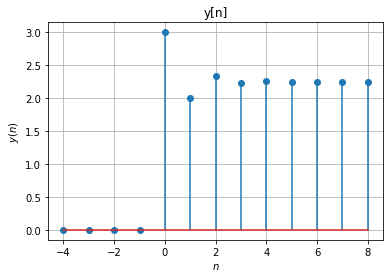
\includegraphics[width=\columnwidth]{y[n].png}
         \caption{Plot of y[n]}
         \label{plot}
\end{figure}
\end{document}
